\documentclass[
  bibliography=totoc,     % Literatur im Inhaltsverzeichnis
  captions=tableheading,  % Tabellenüberschriften
  titlepage=firstiscover, % Titelseite ist Deckblatt
]{scrartcl}

% Paket float verbessern
\usepackage{scrhack}

% Warnung, falls nochmal kompiliert werden muss
\usepackage[aux]{rerunfilecheck}

% unverzichtbare Mathe-Befehle
\usepackage{amsmath}
% viele Mathe-Symbole
\usepackage{amssymb}
% Erweiterungen für amsmath
\usepackage{mathtools}

% Fonteinstellungen
\usepackage{fontspec}
% Latin Modern Fonts werden automatisch geladen
% Alternativ:
%\setromanfont{Libertinus Serif}
%\setsansfont{Libertinus Sans}
%\setmonofont{Libertinus Mono}
\recalctypearea % Wenn man andere Schriftarten gesetzt hat,
% sollte man das Seiten-Layout neu berechnen lassen

% deutsche Spracheinstellungen
\usepackage{polyglossia}
\setmainlanguage{german}


\usepackage[
  math-style=ISO,    % ┐
  bold-style=ISO,    % │
  sans-style=italic, % │ ISO-Standard folgen
  nabla=upright,     % │
  partial=upright,   % ┘
  warnings-off={           % ┐
    mathtools-colon,       % │ unnötige Warnungen ausschalten
    mathtools-overbracket, % │
},                       % ┘
]{unicode-math}

% traditionelle Fonts für Mathematik
\setmathfont{Latin Modern Math}
% Alternativ:
%\setmathfont{Libertinus Math}

\setmathfont{XITS Math}[range={scr, bfscr}]
\setmathfont{XITS Math}[range={cal, bfcal}, StylisticSet=1]

% Zahlen und Einheiten
\usepackage[
locale=DE,                   % deutsche Einstellungen
separate-uncertainty=true,   % immer Fehler mit \pm
per-mode=symbol-or-fraction, % / in inline math, fraction in display math
]{siunitx}

% chemische Formeln
\usepackage[
version=4,
math-greek=default, % ┐ mit unicode-math zusammenarbeiten
text-greek=default, % ┘
]{mhchem}

% richtige Anführungszeichen
\usepackage[autostyle]{csquotes}

% schöne Brüche im Text
\usepackage{xfrac}

% Standardplatzierung für Floats einstellen
\usepackage{float}
\floatplacement{figure}{htbp}
\floatplacement{table}{htbp}

% Floats innerhalb einer Section halten
\usepackage[
section, % Floats innerhalb der Section halten
below,   % unterhalb der Section aber auf der selben Seite ist ok
]{placeins}

% Seite drehen für breite Tabellen: landscape Umgebung
\usepackage{pdflscape}

% Captions schöner machen.
\usepackage[
  labelfont=bf,        % Tabelle x: Abbildung y: ist jetzt fett
  font=small,          % Schrift etwas kleiner als Dokument
  width=0.9\textwidth, % maximale Breite einer Caption schmaler
]{caption}
% subfigure, subtable, subref
\usepackage{subcaption}

% Grafiken können eingebunden werden
\usepackage{graphicx}
% größere Variation von Dateinamen möglich
\usepackage{grffile}

% schöne Tabellen
\usepackage{booktabs}

% Verbesserungen am Schriftbild
\usepackage{microtype}

% Literaturverzeichnis
\usepackage[style=alphabetic,]{biblatex}
% Quellendatenbank
\addbibresource{lit.bib}
\addbibresource{programme.bib}

% Hyperlinks im Dokument
\usepackage[
  unicode,        % Unicode in PDF-Attributen erlauben
  pdfusetitle,    % Titel, Autoren und Datum als PDF-Attribute
  pdfcreator={},  % ┐ PDF-Attribute säubern
  pdfproducer={}, % ┘
]{hyperref}
% erweiterte Bookmarks im PDF
\usepackage{bookmark}

% Trennung von Wörtern mit Strichen
\usepackage[shortcuts]{extdash}

\title{V27: Der Zeeman-Effekt}
\author{
  Simon Schulte
  \texorpdfstring{
    \\
    \href{mailto:simon.schulte@udo.edu}{simon.schulte@udo.edu}
  }{}
  \texorpdfstring{\and}{, }
  Tim Sedlaczek
  \texorpdfstring{
    \\
    \href{mailto:tim.sedlaczek@udo.edu}{tim.sedlaczek@udo.edu}
  }{}
}
\publishers{TU Dortmund – Fakultät Physik}

\date{Durchführung: 11.07.2018\\
      Abgabe: 24.08.2018}


\begin{document}

\maketitle
\thispagestyle{empty}
\setcounter{page}{1}
\pagenumbering{arabic}
\section{Theorie}
Wenn Atome von einem Magnetfeld beeinflusst werden, tritt der Zeeman-Effekt auf.
Dadurch ändern sich die Energieniveaus des jeweiligen Atoms. \\
\\
Experimentell lässt sich die Verschiebung über die Aufspaltung und Polarisation
der durch die Atome emittierten Spektrallinien untersuchen. Über sogenannte
Auswahlregeln lassen sich in der Theorie Vorhersagen über die Energie und
Polarisation der emittierten Strahlung machen.
%
\subsection{Drehimpuls und magnetisches Moment eines Elektrons}
%
Jedes Hüllenelektron besitzt zwei Drehimpulse, den Bahndrehimpuls~$\vec{l}$ und
den Spin~$\vec{s}$. Die Lösungen der quantenmechanischen Eigenwertgleichungen
liefern für die Beträge der Drehimpulse:
%
\begin{align}
    \lvert\,\vec{l}\,\rvert&=\sqrt{l(l+1)}\,\hbar\quad\text{mit}\quad l=0,1,2,\ldots,n-1
    \shortintertext{und}
    \lvert\,\vec{s}\,\rvert&=\sqrt{s(s+1)}\,\hbar\quad\text{mit}\quad s=\frac{1}{2}.
\end{align}
%
Die Drehimpulse bedingen je ein magnetisches Moment. Der Bahndrehimpuls liefert
%
\begin{gather}
    \vec{\mu}_l=-\mu_{\mathup{B}}\sqrt{l(l+1)}\,\vec{l}_0
    \intertext{mit dem Bohrschen Magneton}
    \mu_{\mathup{B}}:=-\frac{e_0\hbar}{2m_0}.
\end{gather}
%
Der Spin liefert
%
\begin{equation}
    \vec{\mu}_s=-g_s\sqrt{s(s+1)}\,\vec{s}_0
\end{equation}
%
mit dem Landé-Faktor~$g_s$ des Elektrons, der etwa den Wert~$2$ hat.
Für den Zustand mit $s=\frac{1}{2}$ und $l=1$ ist $\vec{\mu}_s$ ungefähr
doppelt so groß wie $\vec{\mu}_l$. Der exakte Wert von $g_s$
ergibt sich aus der relativistischen Theorie des Elektrons nach Dirac.

\subsection{Wechselwirkungen der Drehimpulse und der magnetischen Momente}
%
Im Folgenden werden die Wechselwirkungen der Drehimpulse eines
Mehrelektronenatoms betrachtet. Die beiden Drehimpulse eines Elektrons
wechselwirken sowohl untereinander, als auch mit den Drehimpulsen anderer
Elektronen in der Hülle. Diese Überlagerung der Wechselwirkungen ist in der
Theorie schwer zu beschreiben. Daher werden 2 Fälle betrachtet. \\
\\
\noindent
\textbf{1. Fall:}
Bei Atomen mit niedriger Kernladungszahl ist die Wechselwirkung zwischen den
Bahndrehimpulsen verschiedener Elektronen so groß, dass sich diese zum
Gesamtbahndrehimpuls~$\vec{L}$ addieren, wobei
%
\begin{align}
    \lvert\,\vec{L}\,\rvert&=\sqrt{L(L+1)}\,\hbar\quad\text{mit}\quad L=0,1,2,\ldots
    \intertext{gilt. Gemäß der gebräuchlichen Notation in der Atomphysik werden die verschiedenen Werte von $L$ aufsteigend mit den Buchstaben $S,P,D,F,\ldots$ gekennzeichnet. Analog zu den Bahndrehimpulsen kombinieren sich auch die Spins der Elektronen additiv zum Gesamtspin~$\vec{S}$. Es gilt}
    \lvert\,\vec{S}\,\rvert&=\sqrt{S(S+1)}\,\hbar\quad\text{mit}\quad S=\frac{N}{2},\frac{N}{2}-1,\ldots,\frac{1}{2},0
\end{align}
%
wobei $N$ die Anzahl der Hüllenelektronen ist.
Auch dem Gesamtbahndrehimpuls~$\vec{L}$ und dem Gesamtspin~$\vec{S}$ wird mit
%
\begin{align}
    \lvert\,\vec{\mu}_L\,\rvert&=\mu_{\mathup{B}}\sqrt{L(L+1)}
    \shortintertext{und}
    \lvert\,\vec{\mu}_S\,\rvert&=g_S\mu_{\mathup{B}}\sqrt{S(S+1)}
\end{align}
%
ein magnetisches Moment zugeordnet.
Für nicht zu starke Magnetfelder ergibt sich ein Gesamtdrehimpuls
%
\begin{gather}
    \vec{J}=\vec{L}+\vec{S}
    \shortintertext{mit}
    \lvert\,\vec{J}\,\rvert=\sqrt{J(J+1)}
\end{gather}
%
wobei $J$ entweder ganz- oder halbzahlig sein kann.
Der obige Zusammenhang wird auch als $LS$-Kopplung oder
Russell-Saunders-Kopplung bezeichnet. $J$ wird üblicherweise als unterer Index
an den Symbolen $S,P,D,F,\ldots$ notiert. Oberer Index ist die Multiplizität $M=2S+1$. \\
\\
\noindent
\textbf{2. Fall:}
Bei schweren Atomen ist die Wechselwirkung zwischen Spin und Bahndrehimpuls
eines Elektrons groß gegenüber der Wechselwirkung der Bahndrehimpulse und Spins
verschiedener Elektronen untereinander. Es ergibt sich der Gesamtdrehimpuls
%
\begin{equation}
    \vec{j}_i=\vec{l}_i+\vec{s}_i
\end{equation}
%
je Einzelektron, sodass kein Gesamtdrehimpuls~$\vec{L}$ und Gesamtspin $\vec{S}$
mehr definiert sind. Die $\vec{j}_i$ addieren sich nun zum Gesamtdrehimpuls $\vec{J}$.
Diese Art der Wechselwirkung wird auch als $j$-$j$-Kopplung bezeichnet.
\noindent
Zwischen den genannten Grenzfällen existiert für mittlere Kernladungszahlen ein
fließender Übergang.
%
\subsection{Aufspaltung der Energieniveaus eines Atoms im homogenen Magnetfeld}
%
Das zu $\vec{J}$ gehörende magnetische Moment ergibt sich zu
%
\begin{equation}
    \vec{\mu}=\vec{\mu}_L+\vec{\mu}_S.
\end{equation}
%
$\vec{J}$ und $\vec{\mu}$ sind im Allgemeinen nicht parallel, doch der
Erwartungswert der zu $\vec{J}$ senkrechten Komponente verschwindet aufgrund
der präzedierenden Bewegung um die Magnetfeldrichtung im zeitlichen Mittel.
Aus der Quantenmechanik folgt
%
\begin{equation}
     \lvert\,\vec{\mu}_J\,\rvert=g_J\mu_{\mathup{B}}\sqrt{J(J+1)}
\end{equation}
%
mit dem Landé-Faktor
%
\begin{equation}
    g_J:=\frac{3J(J+1)+S(S+1)-L(L+1)}{2J(J+1)}.
    \label{eq:g_J}
\end{equation}
%
Ein weiteres Resultat der Quantenmechanik ist die Richtungsquantelung im
homogenen Magnetfeld. Es gilt:
%
\begin{equation}
    \mu_{J_z}=-mg_J\mu_{\mathup{B}}
\end{equation}
%
mit der Orientierungsquantenzahl $m\in\{-J,-J+1,\ldots,J-1,J\}$.
Daraus folgen $2J+1$ Einstellmöglichkeiten für ein magnetisches Moment in einem
äußeren Magnetfeld. Für die Energie, die ein Moment $\vec{\mu}$ im Magnetfeld
erhält, ergibt sich:
%
\begin{equation}
    E_{\mathup{mag}}=-\vec{\mu}\vec{B}=mg_J\mu_{\mathup{B}}B.
    \label{eq:E_mag}
\end{equation}
%
Das Energieniveau $E_0$ im feldfreien Raum spaltet bei $B\neq0$ in $2J+1$
äquidistante Niveaus auf. Beispielhaft ist dies in Abbildung
\ref{fig:aufspaltung} für ein Atom mit $J=2$ skizziert. Die Aufspaltung
ermöglicht neue Übergänge zwischen Energieniveaus und somit neue Spektrallinien.
Dieser Effekt wird als Zeeman-Effekt bezeichnet.
%
\begin{figure}
    \centering
    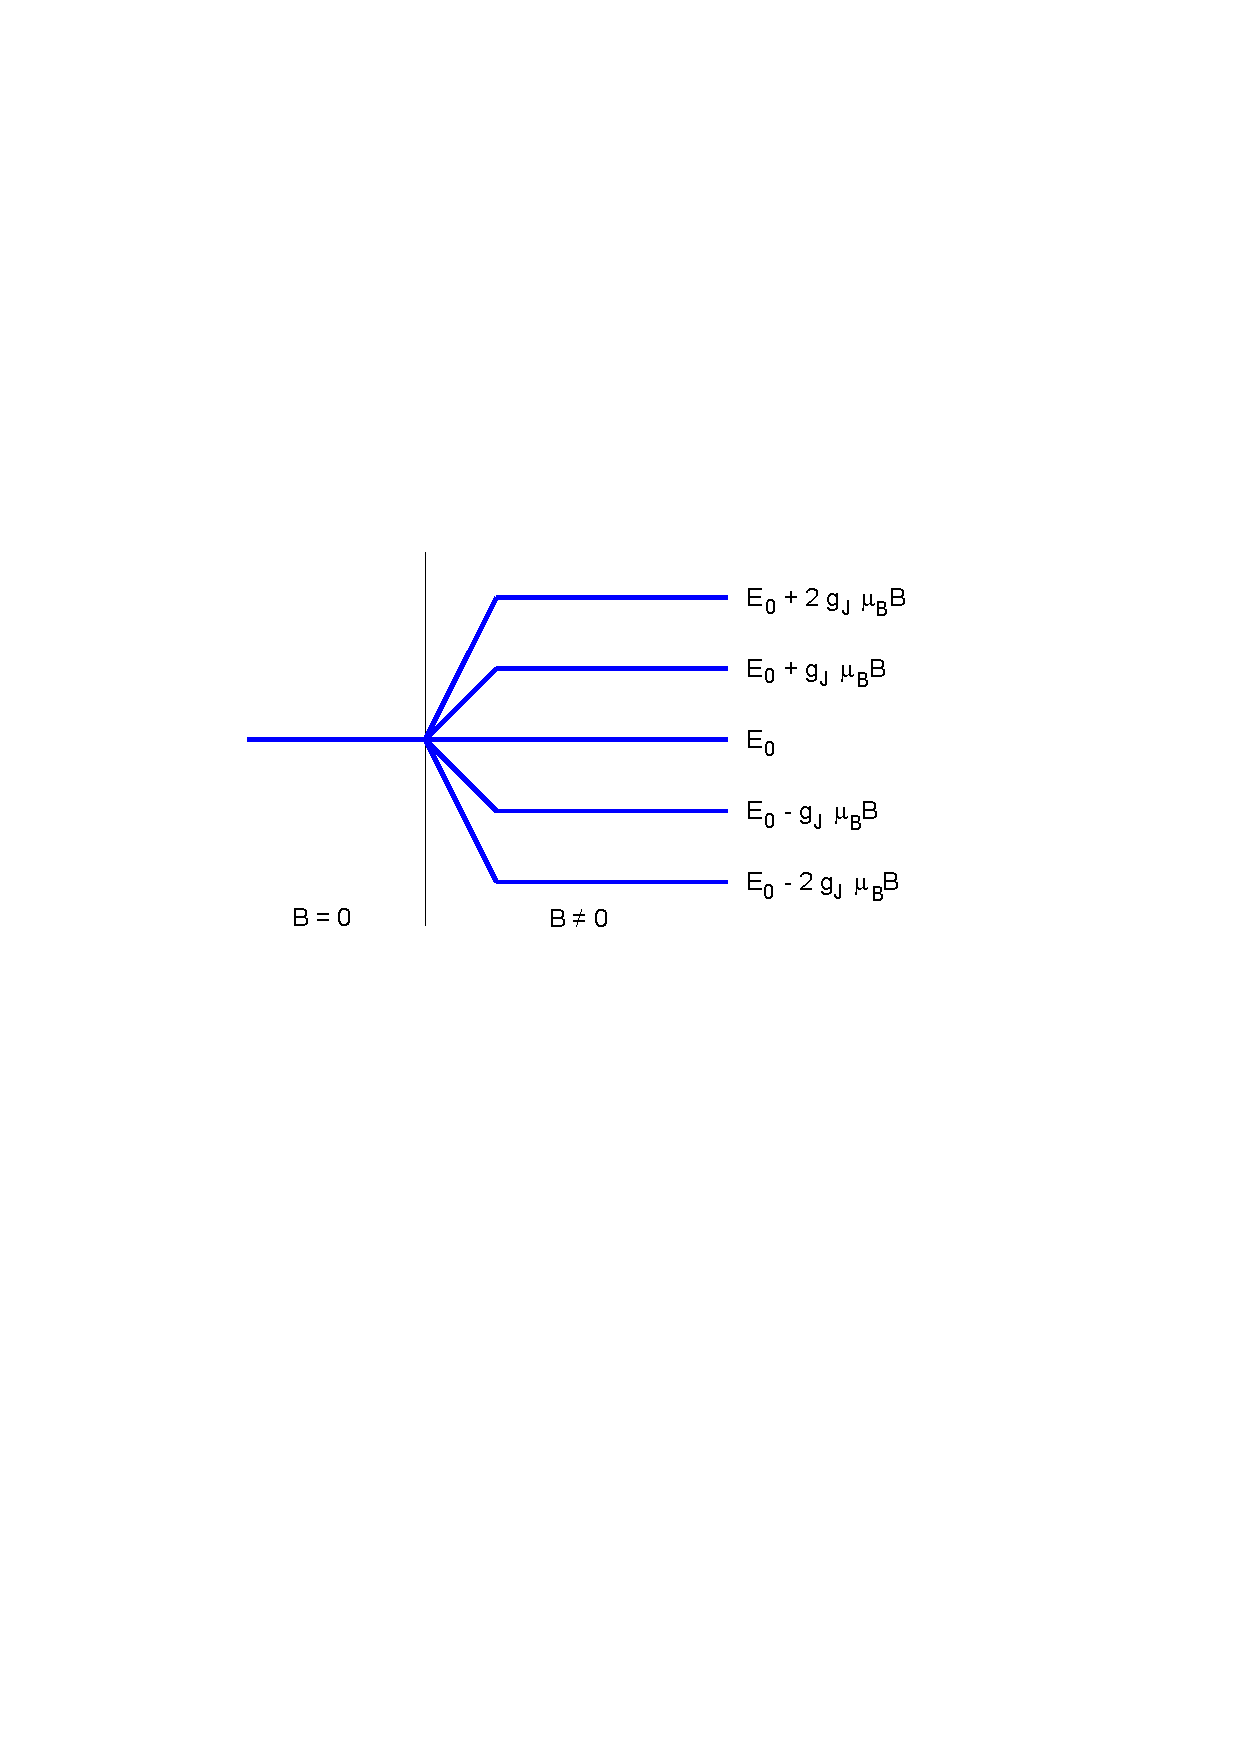
\includegraphics[width=0.6\textwidth]{aufspaltung.pdf}
    \caption{Schematische Darstellung der Aufspaltung eines Energieniveaus eines Atoms mit Gesamtdrehimpulsquantenzahl $J=2$.\cite{V27}}
    \label{fig:aufspaltung}
\end{figure}
%
\subsection{Der Zeeman-Effekt}
%
Da in der zeitabhängigen Schrödingergleichung der Spin nicht berücksichtigt wird,
sind die bisherigen Ergebnisse nur für den Fall $S = 0$ gültig. Dies nennt man
den Normalen Zeeman-Effekt. In diesem Fall gilt für
alle $J$, dass $g_J = 1$ ist. Folglich sind die Aufspaltungen unabhängig von den
Quantenzahlen.
\begin{figure}
  \centering
  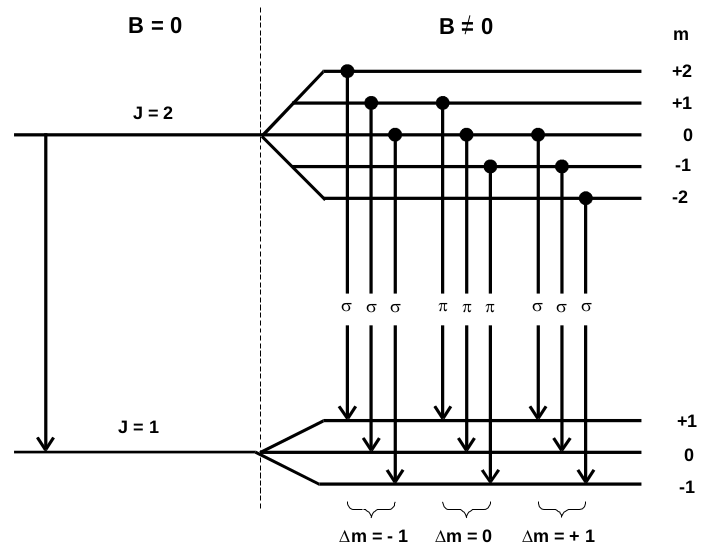
\includegraphics[scale=0.4]{normal.png}
  \caption{Aufspaltung der Energieniveaus und zugehörige Polarisation für den
  normalen Zeeman-Effekt. \cite{anleitung}}
  \label{fig:1}
\end{figure}
Ein Beispiel für eine solche Aufspaltung ist in Abbildung \ref{fig:1} zu sehen.
Dabei ist zu sehen, dass die Energieniveaus äquidistant sind. Es ergibt sich
\begin{equation}
  E_{\symup{mag}}= m \, \mu_B \, B \, .
  \label{eqn:10}
\end{equation}
Die Aufspaltungslinien lassen sich den Auswahlregeln zuordnen, was auch in
Abbildung \ref{fig:1} dargestellt ist. Allerdings sind je nach Beobachtungsrichtung
wegen der unterschiedlichen Polarisation nicht alle Linien zu sehen. Die $\pi$-Linie
(zu $\symup \Delta m = 0$) ist nur sichtbar, wenn die Beobachtungsrichtung
senkrecht zur Feldrichtung, also transversal, ist. Außerdem ist sie gegenüber
der feldfreien Linie nicht verschoben, im Gegensatz zu den Linien mit $\symup \Delta m = \pm 1$,
da sich die Energie um $\mu_B \, B$ im Vergleich zum feldfreien Fall unterscheidet.
Weil sie zirkular polarisiert sind, erscheinen sie bei transversaler Beobachtung als
linear polarisiert.
Der andere Fall, also $S \neq 0$, wird Anomaler Zeeman-Effekt genannt.
Die Auswahlregeln sind auch in diesem Fall noch gültig. Dies lässt
sich über die spinabhängige Schrödingergleichung zeigen. Die Auspaltung wird
vielfältiger, da $g$ nicht mehr für alle $J=1$ ist, sondern von $L, S$ und $J$
abhängt.
\section{Durchführung}
\subsection{Versuchsaufbau}
\begin{figure}
  \centering
  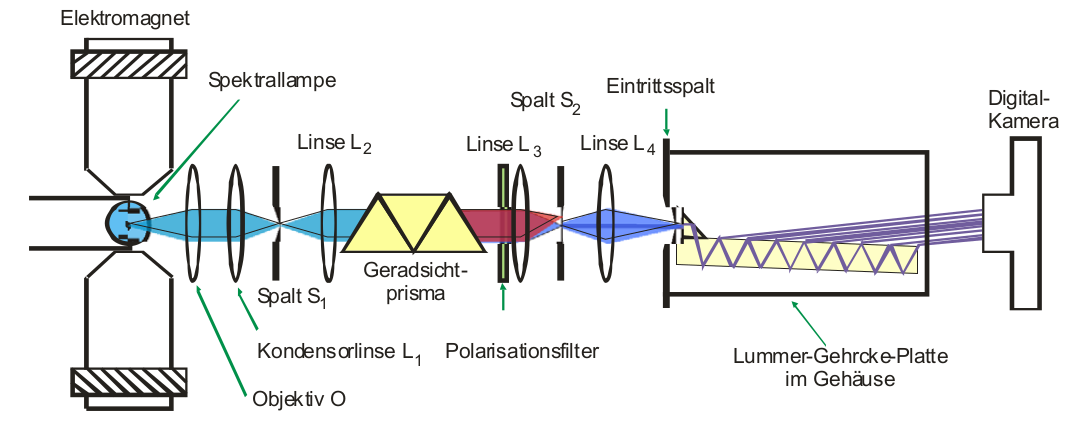
\includegraphics[scale=0.39]{aufbau.png}
  \caption{Der verwendendete Versuchsaufbau.}
  \label{fig:3}
\end{figure}
\noindent
Abbildung \ref{fig:3} zeigt den verwendeten Versuchsaufbau. Das Licht der
verwendeten Cd-Lampe wird in rote und blaue Linien aufgespaltet. Dafür wird die
Lampe in einen starken Elektromagnet gestellt. Dann
wird transversal zum Magnetfeld das Licht nach Wellenlängen aufgespalten. Dies
geschieht durch Linsen, Spalte und ein Geradsichtprisma. Nun kann durch einen
Spalt und einen Polarisationsfilter die gewünschte Linie mit der gewünschten
Polarisation ausgewählt und auf eine Lummer-Gehrke-Platte abgebildet werden.
Dadurch entsteht ein Interferenzmuster. Dieses wird über eine Digitalkamera
aufgenommen. Bei monochromatischem Licht erzeugt die Lummer-Gehrke-Platte
Gangunterschiede von $\lambda$, was die eingestrahlte Wellenlänge ist. Beim
Einschalten des Magnetfeldes tritt eine Verschiebung der Wellenlänge um
$\symup{\Delta} \lambda$ auf, welche wiederum die interferierten Strahlen
um $\symup{\Delta} s$ verschiebt. Dabei wird das Dispersionsgebiet
\begin{equation}
    \symup \symup{\Delta} \lambda_D = \frac{\lambda^2}{2\, d} \cdot \sqrt{\frac{1}{n^2 - 1}}
    \label{eqn:11}
\end{equation}
nicht überschritten, da sonst eine Überlagerung der Wellenlängen auftreten würde.
Hierbei ist $d$ die Dicke der Platte und $n$ die Ordnung des Maximums. Das
Auflösungsvermögen $A$ der Lummer-Gehrke-Platte lässt sich beschreiben durch:
\begin{equation}
  A = \frac{L}{\lambda} (n^2 - 1).
  \label{eqn:12}
\end{equation}\
Dabei entspricht $L$ der Länge der Platte und $n$ dem Brechungsindex.
\subsection{Versuchsdurchführung}
Als erstes wird der Elektromagnet, indem das B-Feld über ein Gaußmeter
in Abhängigkeit von dem Feldstrom gemessen wird in einem Intervall von
$0 \leq I \leq \SI{20}{\ampere}$ geeicht.
Daraufhin wird der Aufbau so justiert, dass die gesuchten Wellenlängen
($\lambda = \SI{480}{\nano\meter}$ und $\lambda = \SI{643.8}{\nano\meter}$)
mit der durch den Polarisationsfilter eingestellten Polarisation auf die
Lummer-Gehrke-Platte fallen. Daraufhin wird eine Digitalkamera genutzt, um
Bilder von Interferenzbildern bei verschiedenen Polarisationen und Magnetfeldstärken
aufzunehmen. Dadurch ergibt sich die Wellenlängenverschiebung.
\end{document}
